% Title     :: SamzaSQL: Scalable Fast Data Management with Streaming SQL
% Author    :: Milinda Pathirage
% Email     :: mpathira@indiana.edu
% Website   :: http://milinda.pathirage.org
% Template  :: sthlm beamer theme by Benjamin Weiss (hendryolson@gmail.com, http://v42.com), 
%              which is HEAVILY based on the HSRM beamer theme created by Benjamin Weiss
%			   (benjamin.weiss@student.hs-rm.de), which can be found on GitHub
%			   <https://github.com/hsrmbeamertheme/hsrmbeamertheme>.



%-=-=-=-=-=-=-=-=-=-=-=-=-=-=-=-=-=-=-=-=-=-=-=-=
%
%        LOADING DOCUMENT
%
%-=-=-=-=-=-=-=-=-=-=-=-=-=-=-=-=-=-=-=-=-=-=-=-=

\documentclass[newPxFont]{beamer}
\usetheme{sthlm}
%\usecolortheme{sthlmv42}

%-=-=-=-=-=-=-=-=-=-=-=-=-=-=-=-=-=-=-=-=-=-=-=-=
%        LOADING PACKAGES
%-=-=-=-=-=-=-=-=-=-=-=-=-=-=-=-=-=-=-=-=-=-=-=-=
\usepackage[utf8]{inputenc}
\usepackage{hyperref}
\usepackage{minted}
\usepackage{xcolor}
\usepackage{tikz}
\usepackage{tikz-qtree}
\usetikzlibrary{trees}
\usepackage{xxcolor}
\usetikzlibrary{shapes.misc,shapes.geometric,shapes.arrows,decorations.pathmorphing,decorations.shapes}
\usetikzlibrary{matrix,chains,scopes,positioning,arrows,fit}
\usepackage{smartdiagram}
\usesmartdiagramlibrary{additions}


\usepackage{chronology}

\renewcommand{\event}[3][e]{%
  \pgfmathsetlength\xstop{(#2-\theyearstart)*\unit}%
  \ifx #1e%
    \draw[fill=black,draw=none,opacity=0.5]%
      (\xstop, 0) circle (.2\unit)%
      node[opacity=1,rotate=45,right=.2\unit] {#3};%
  \else%
    \pgfmathsetlength\xstart{(#1-\theyearstart)*\unit}%
    \draw[fill=black,draw=none,opacity=0.5,rounded corners=.1\unit]%
      (\xstart,-.1\unit) rectangle%
      node[opacity=1,rotate=45,right=.2\unit] {#3} (\xstop,.1\unit);%
  \fi}%

\newcommand{\specialcell}[2][l]{%
  \begin{tabular}[#1]{@{}l@{}}#2\end{tabular}}

%-=-=-=-=-=-=-=-=-=-=-=-=-=-=-=-=-=-=-=-=-=-=-=-=
%        BEAMER OPTIONS
%-=-=-=-=-=-=-=-=-=-=-=-=-=-=-=-=-=-=-=-=-=-=-=-=

%\setbeameroption{show notes}

%-=-=-=-=-=-=-=-=-=-=-=-=-=-=-=-=-=-=-=-=-=-=-=-=
%
%	PRESENTATION INFORMATION
%
%-=-=-=-=-=-=-=-=-=-=-=-=-=-=-=-=-=-=-=-=-=-=-=-=

\title{Horme}
\subtitle{Random Access Big Data Analytics}
%\date{\small{\jobname}}
%\date{\today}
\author{Guangchen Ruan, Beth Plale; \emph{Milinda Pathirage (Presenter)}}
\institute{School of Informatics and Computing, Indiana University}

\hypersetup{
pdfauthor = {Milinda Pathirage: milinda.pathirage@gmail.com},
pdfsubject = {},
pdfkeywords = {},
pdfmoddate= {D:\pdfdate},
pdfcreator = {}
}

\begin{document}
\setbeamertemplate{caption}{\raggedright\insertcaption\par}

%-=-=-=-=-=-=-=-=-=-=-=-=-=-=-=-=-=-=-=-=-=-=-=-=
%
%	TITLE PAGE
%
%-=-=-=-=-=-=-=-=-=-=-=-=-=-=-=-=-=-=-=-=-=-=-=-=

\maketitle

%\begin{frame}[plain]
%	\titlepage
%\end{frame}

%-=-=-=-=-=-=-=-=-=-=-=-=-=-=-=-=-=-=-=-=-=-=-=-=
%
%	TABLE OF CONTENTS: OVERVIEW
%
%-=-=-=-=-=-=-=-=-=-=-=-=-=-=-=-=-=-=-=-=-=-=-=-=

\section{Introduction}

%-=-=-=-=-=-=-=-=-=-=-=-=-=-=-=-=-=-=-=-=-=-=-=-=
%	FRAME:
%-=-=-=-=-=-=-=-=-=-=-=-=-=-=-=-=-=-=-=-=-=-=-=-=
\begin{frame}[c]{Hathitrust Research Center (HTRC)}
Research arm of \textbf{Hathitrust Digital Library} that develops and maintain infrastructure for enabling computational access to \textbf{14 million} digitized volumes.

\vspace{1em}

\begin{exampleblock}{Mission}
Enable researchers world-wide to accomplish tera-scale text data-mining and analysis  
\end{exampleblock}
\end{frame}

\begin{frame}[c]{HTRC Analytics Workflow}
\smartdiagramset{back arrow disabled=true,
additions={
additional item offset=1em,
additional item height=0em,
additional item text width=15em,
additional arrow color=teal!40,
additional arrow line width=4pt,
additional connections disabled=false,
   additional arrow color=red,
   additional arrow tip=stealth,
   additional arrow line width=1pt
   }}
\smartdiagramadd[flow diagram:horizontal]{Search Solr,
  Create Workset, Get Volumes, Analyse}{above of module2/{Workset is given as an input to analytic sub-systems that downloads volumes from storage sub-systems integrated to them},
  below of module1/{Select a subset of data for analysis},
  below of module3/{Random access to the corpus}}
\end{frame}

\begin{frame}[c]{HTRC Analytics Infrastructure}


% Based on http://tex.stackexchange.com/questions/125234/upside-down-tikz-qtree-with-concentrated-edges

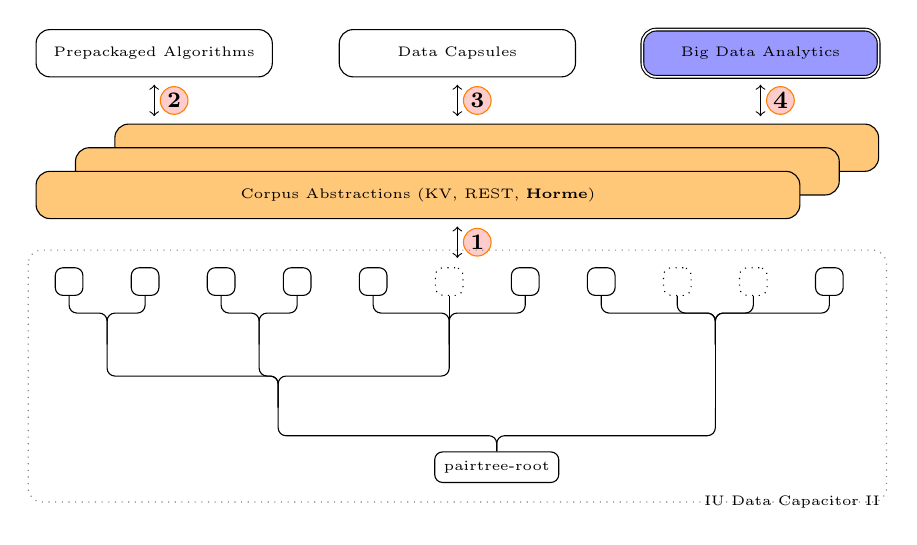
\begin{tikzpicture}
[   grow'=up,
    level distance=.8cm,
    sibling distance=.6cm,
    edge from parent fork up,
    edge from parent/.style={draw,rounded corners=1mm}
]
\begin{scope}[local bounding box=scope1]
  \draw[rounded corners=5pt] (-6.7,4.8) rectangle (-3.7,4.2) node[pos=.5] {\tiny Prepackaged Algorithms};
  \draw[rounded corners=5pt] (-2.85,4.8) rectangle (0.15,4.2) node[pos=0.5] {\tiny Data Capsules};
  \draw[rounded corners=5pt,fill=blue!40,double] (1,4.8) rectangle (4,4.2) node[pos=0.5] {\tiny Big Data Analytics};
  \draw[fill={rgb:orange,1;yellow,2;pink,5},rounded corners=5pt] (-5.7,3.6) rectangle (4,3) ;
  \draw[fill={rgb:orange,1;yellow,2;pink,5},rounded corners=5pt] (-6.2,3.3) rectangle (3.5,2.7) ;
  \draw[fill={rgb:orange,1;yellow,2;pink,5},rounded corners=5pt] (-6.7,3) rectangle (3,2.4) node[pos=.5] {\tiny Corpus Abstractions (KV, REST, \textbf{Horme})};
\end{scope}
\draw[<->] (-1.35,2.3) -- (-1.35,1.9) node[draw=orange,anchor=west,pos=0.5,circle,fill=red!20,inner sep=0pt,minimum size=10pt,xshift=2pt]{\footnotesize \textbf{1}};
\draw[<->] (-5.2,4.1) -- (-5.2,3.7) node[draw=orange,anchor=west,pos=0.5,circle,fill=red!20,inner sep=0pt,minimum size=10pt,xshift=2pt]{\footnotesize \textbf{2}};
\draw[<->] (-1.35,4.1) -- (-1.35,3.7) node[draw=orange,anchor=west,pos=0.5,circle,fill=red!20,inner sep=0pt,minimum size=10pt,xshift=2pt]{\footnotesize \textbf{3}};
\draw[<->] (2.5,4.1) -- (2.5,3.7) node[draw=orange,anchor=west,pos=0.5,circle,fill=red!20,inner sep=0pt,minimum size=10pt,xshift=2pt]{\small \textbf{4}};
\begin{scope}[shift={($(scope1.north)+(0.5cm,-5.6cm)$)}]
  \tikzstyle{var} = [draw,shape=rectangle,minimum size=1em,rounded corners=1mm]
  \tikzstyle{operator} = [draw=none,fill=none,above,pos=0]
  \tikzset{every node/.style={var}}
  \Tree [.\tiny pairtree-root 
            [\edge node[operator] {};
            [
              [.\node[] {}; ] [.\node[] {}; ]
             ] [ [.\node[] {}; ][.\node[] {}; ]] [ [.\node[] {}; ][.\node[dotted] {}; ][.\node[] {}; ] ]
          ]
          [ [[.\node[] {}; ] [.\node[dotted] {}; ] [.\node[dotted] {}; ] [.\node[] {}; ]] 
          ]
        ]
\end{scope}
\draw[rounded corners=5pt,dotted,gray] (-6.8,2) rectangle (4.1,-1.2) node[draw=none,fill=none,pos=1,xshift=-1.2cm,black] {\tiny IU Data Capacitor II};
\end{tikzpicture}
\end{frame}

\section{Motivation}

\begin{frame}[c]{Hadoop on HPC and HTC Environments}
\begin{figure}[t]
  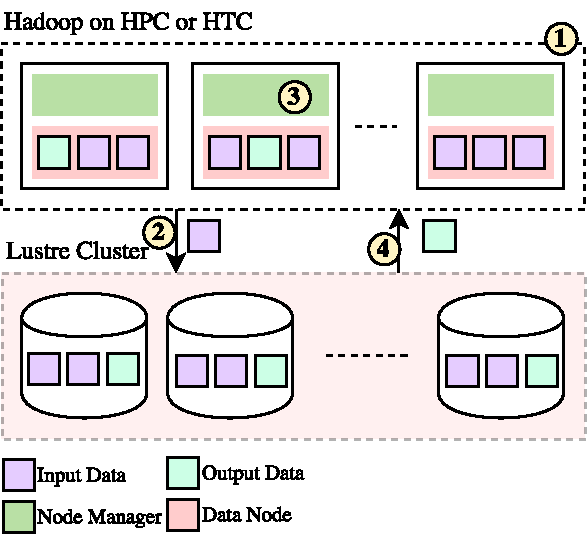
\includegraphics[scale=0.7]{hadoop-on-hpc-2}
  \centering
\end{figure}
\end{frame}

\begin{frame}[c]{Hadoop on HPC and HTC Environments}
  \begin{itemize}
    \item Data is stored in a \emph{parallel file system (PFS)} such as Lustre connected to compute nodes via network
    \item Often data get staged to the scratch space in compute nodes (e.g. HDFS data nodes) from Lustre before the actual computation
    \item Results get copied back to Lustre after job completion
    \item \textbf{High data staging overhead}
    \item HDFS on HPC and HTC environments is limited by scratch space capacity of compute nodes
  \end{itemize}
\end{frame}

\begin{frame}[c]{Text Data Mining on HPC and HTC Environments}
  \begin{itemize}
    \item Use Solr search or some other means to narrow down the set of digitized texts to analyse
    \item Apply text mining techniques such as topic modeling on the selected subset
    \item Often this subset is randomly distributed across the corpus (Around 14 million volumes in HTRC)
    \item HDFS performs poorly in random access use cases
    \item HBase is good for random access, but needs to deploy external to HPC or HTC compute nodes due to transient nature of batch jobs
    \item HBase over Lustre is not optimal
  \end{itemize}
\end{frame}

\section{Horme}

\begin{frame}[c]{Horme}
\begin{itemize}
  \item Indexed binary file format for packing key/value pairs where size of the value range from couple of kilobytes to couple of mega bytes
  \item A Set of tools for packing and managing key/value pairs   
  \item Storage extensions for popular Big Bidata processing frameworks to read and write Hrome binary files
  \item Not tied to any processing framework
  \item Works on top of any file system
  \item Delegates replication, file striping and fault-tolerance to underline file system
\end{itemize}
\end{frame}

\begin{frame}[c]{Horme - BloomHashIndexFile}
\begin{figure}[t]
  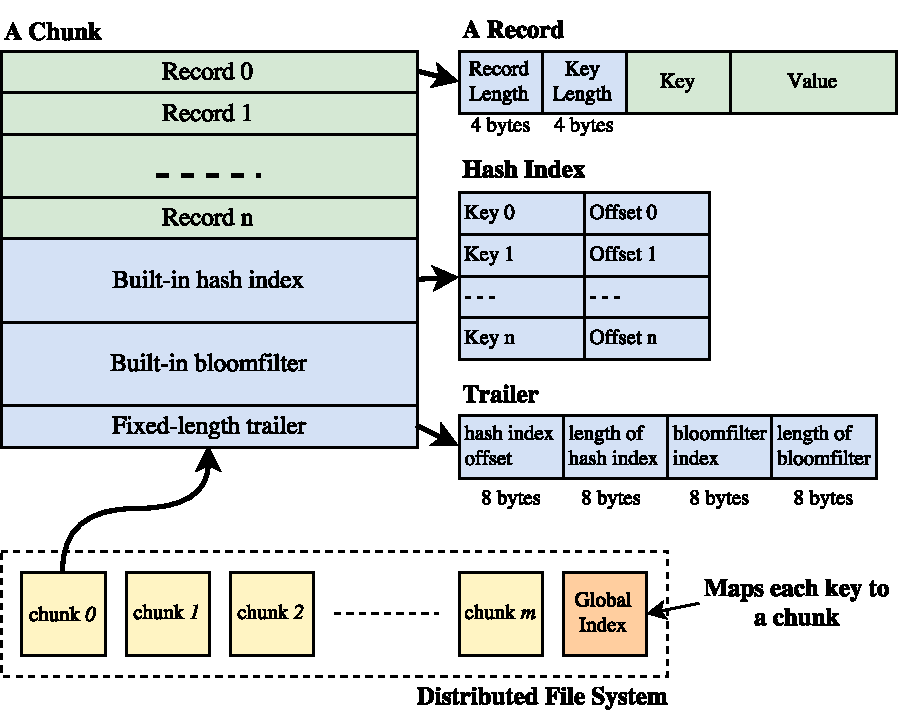
\includegraphics[scale=0.6]{horme-2}
  \centering
\end{figure}  
\end{frame}

\begin{frame}[c]{Horme - Programming Abstraction}
  \begin{itemize}
    \item Reader
    \begin{center}
      \begin{tabular}{| l | l |}
       \hline
       \textbf{Scan} & \texttt{for(Record r : BloomHashIndexFile)} \\ 
       \hline
       \textbf{Random Access} & \texttt{Record get(Key key)} \\  
       \hline
       \textbf{Membership Test} & \texttt{boolean probablyHasKey(Key key)} \\    
       \hline
       \textbf{Accessors} & \specialcell{\texttt{HashIndex getHashIndex()} \\ 
\texttt{BloomFilter getBloomFilter()}} \\    
       \hline
      \end{tabular}
    \end{center}
    \item Writer
    \begin{center}
      \begin{tabular}{| l | l |}
       \hline
       \textbf{Write} & \texttt{void append(Key key, Value val)} \\ 
       \hline
       \textbf{Misc.} & \texttt{int getLength()} \\  
       \hline
      \end{tabular}
    \end{center}
  \end{itemize}
\end{frame}

\begin{frame}[c]{Horme - Distributed Packing Utility}
  \begin{itemize}
    \item Pack Key/Value style raw data to binary chunks
    \item Embarrasingly parallel packing process
    \item For the sake of load balancing each chunk should carray roughly the same payload
    \begin{itemize}
      \item Same \# of records (e.g., simulation analysis task)
      \item Same chunk file size (e.g., text mining task)
    \end{itemize}
  \end{itemize}
\end{frame}

\begin{frame}[c]{Horme - Parallel Processing Layer}
  \begin{itemize}
    \item Hadoop input and output format extension on top of BloomHashIndexFile
    \item Retains MapReduce Key/Value semantics 
    \item Support both scan and random access 
    \item Binary chunks can be served from a network file system or a HDFS cluster coupled with Hadoop deployment
  \end{itemize}
\end{frame}

\begin{frame}[c]{Horme - Processing Chunks from Network Storage}
\begin{figure}[t]
  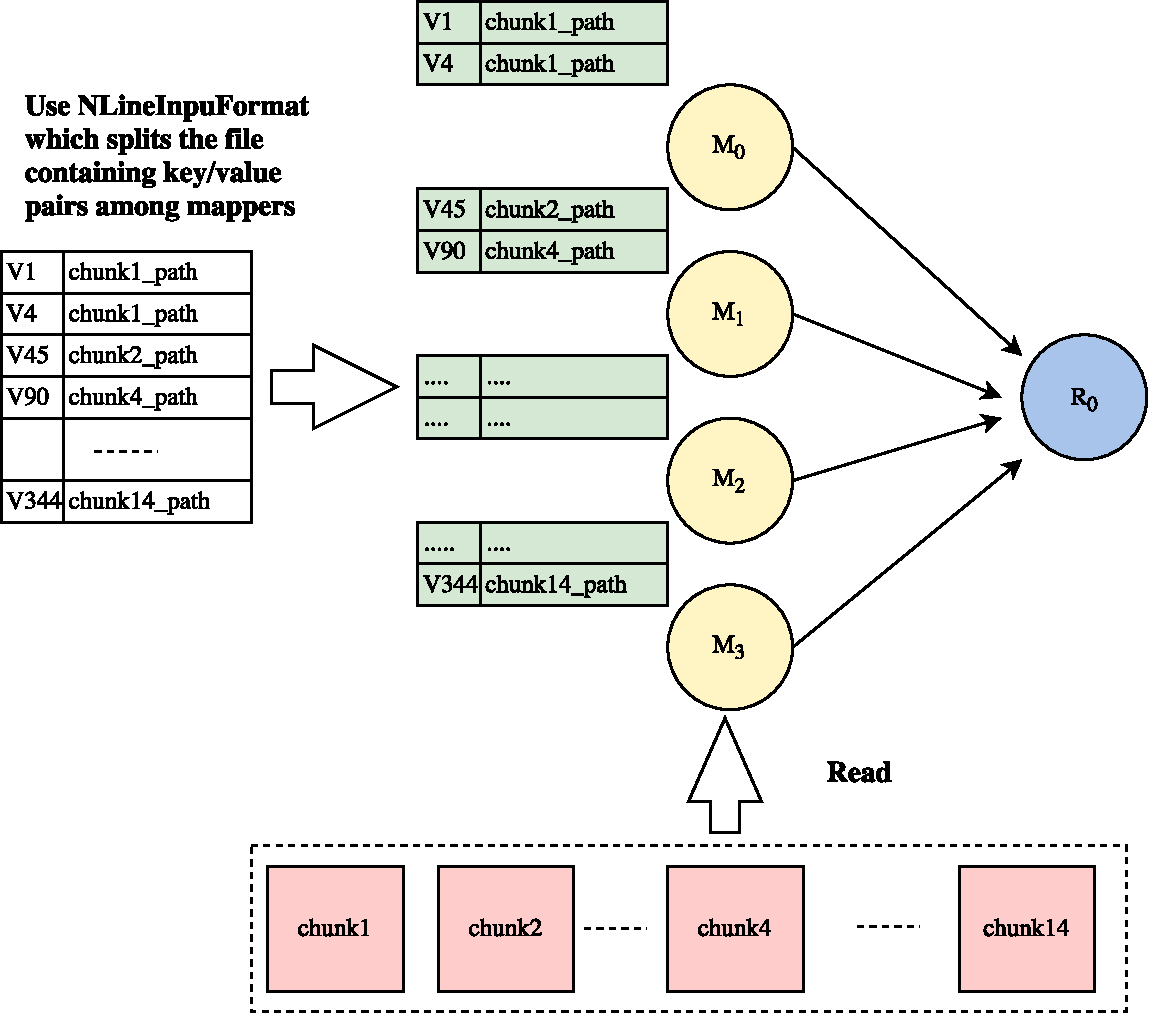
\includegraphics[scale=0.4]{horme-with-pfs}
  \centering
\end{figure}
\end{frame}

\begin{frame}[c]{Horme - Processing Chunks from Network Storage}
\begin{itemize}
  \item With NLineInputFormat, a single input split consists of N consecutive lines
  \item \texttt{BloomHashIndexFile}'s \texttt{Reader} is used to read the value corresponding to each key in input split at mapper
  \item Input should be sorted by binary chunk's path so that the \texttt{RecordReader} only needs to opens a new file when the next line is a new chunk
  \item Workload is balanced with respect to number of records processed
  \item Workload is approximately balances with respect to the size of the records 
\end{itemize}
\end{frame}

\begin{frame}[c]{}
  
\end{frame}
\end{document}